\section{Theory}
In this repport we are working with the Fresnel relations, which describe the
amount of $s$- and $p$-polarized light transmitted and reflected at the
boundary of a dielectric surface. Generally we remind ourself of the relation
between the angles of the incoming light $\theta_i$, the reflected light
$\theta_r$ and refracted (also called transmitted) light $\theta_t$. The angles
are measured from the normal of the dielectric surface (see \cref{fig:angles}).
The relation between the incoming and reflected beam is given by the simple
relation\footnote{This is the only solution for the given boundary conditions at the surface and
as the light propagates in the same material, and hence has the same index of
refraction.}:
%
\begin{align}
    \theta_i = \theta_r,
\end{align}
%
The relation between the angles of incidence and refraction is given by Snells' law:%
\begin{align}
n_1\sin{\theta_i}=n_2\sin{\theta_t}
\end{align}
%
where $n_1$ and $n_2$ are the refractive indices of the materials at the boundary of the incoming and reflected light beam. 
\begin{figure}[h!]
    \centering
    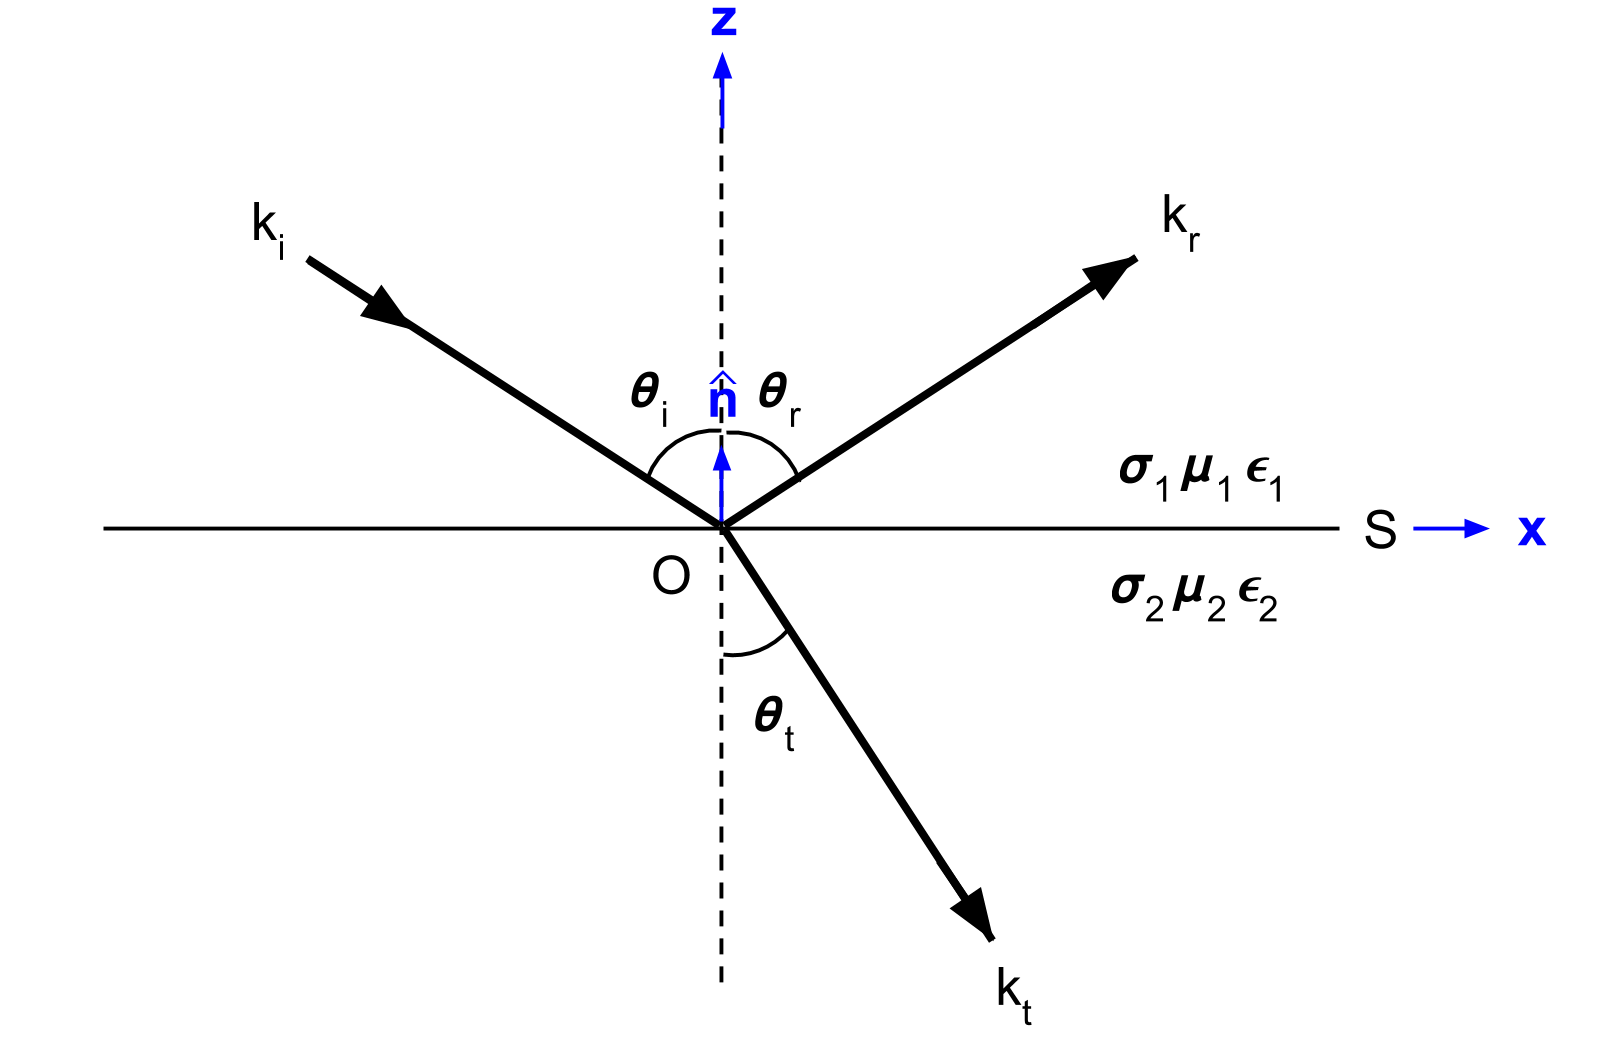
\includegraphics[width=\columnwidth]{snellslaw}
    \caption{Incomming light beam at angle $\theta_i$ to the
        plane of incidence reflected and refracted
        at angles $\theta_r$ and $\theta_t$ respectively. Here $k$ is the
    orientation of the propagation.
    }\label{fig:angles}
\end{figure}

\subsection{Polarization}
The plane spanned by the normal vector to our dielectric surface $\hat{\textbf{n}}$ and the wave vector $\textbf{k}_i$, which is in the direction of the propagation of the incomming light, is called \textit{the plane of incidence} (see \cref{fig:plane}). The direction of the $\textbf{E}$-field relative to this plane then determines the polarization of the light, if $\textbf{E}$ is parallel to the plane of incidence the light is $p$-polarized and if $\textbf{E}$ is perpendicular to the plane of incidence then the light is $s$-polarized. 
%
\noindent
Light from normal light sources has a mixture of all possible directions of polarization but generally any polarization can be given as a linear combination in a basis of electric field with $s$- and $p$-polarization. Using a polarizer one can filter one kind of polarization of a beam.
\begin{figure}[h]
    \centering
    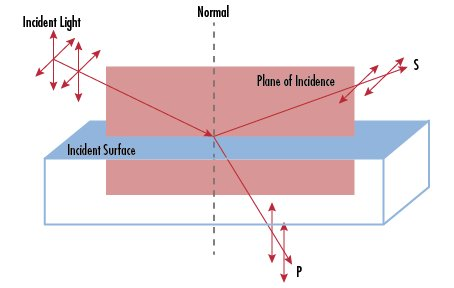
\includegraphics[width=\columnwidth]{plane}
    \caption{Plane of incidence, spanned out by the normal to the incident surface and the direction vector of the beam.}
    \label{fig:plane}
\end{figure}

\subsection{Fresnel relations}
When a beam of light interacts with the surface of a dielectricum a certain percentage of the light will be reflected as well as transmitted. The percentage of light reflected is denoted $R$ and the percentage transmitted is denoted $T$. As the light is either transmitted or reflected it is natural to conclude that:
%
\begin{align}
R+T=1
\end{align}
%
To make things easier for ourselves we define $R=r^2$ and $T=\frac{n_2\cos{\theta_t}}{n_1\cos{\theta_r}}t^2$ where $r=\frac{E_1'}{E_1}$ and  $t=\frac{E_2}{E_1}$ with $E_1$ denoting the magnitude of the incoming $\textbf{E}$-field, $E_1'$ denoting the magnitude of the reflected $\textbf{E}$-field and $E_2$ denoting the magnitude of the transmitted $\textbf{E}$-field. As the direction of the $\textbf{E}$-field can be written in the basis of $s$- and $p$-polarization we can define our reflection and transmission indexes for $p$- and $s$-polarized light seperately. Our $r_p,r_s,t_p$ and $t_s$ given as functions of $\theta_r$ and $\theta_t$ are:

%Find more details
\begin{align}
r_p = & \frac{n_{2}\cos(\theta_r)-n_1\cos(\theta_t)}{n_2\cos(\theta_r)+n_1\cos(\theta_t)} = \frac{\tan(\theta_r-\theta_t)}{\tan(\theta_r+\theta_t)}\\
%
t_p = & \frac{2n_1\cos(\theta_r)}{n_2\cos(\theta_r)+n_2\cos(\theta_t)} 
= \frac{2\cos(\theta_r)\sin(\theta_t)}{\sin(\theta_r+\theta_t)\cos(\theta_r+\theta_t)}
\end{align}

\begin{align}
r_s = & \frac{n_1\cos(\theta_r)-n_2\cos(\theta_t)}{n_1\cos(\theta_r)+n_2\cos(\theta_t)}= -\frac{\sin(\theta_r-\theta_t)}{\sin(\theta_r+\theta_t)}\\
%
t_s = & \frac{2n_1\cos(\theta_r)}{n_1\cos(\theta_r)+n_2\cos(\theta_t)} = \frac{2\cos(\theta_r)\sin(\theta_t)}{\sin(\theta_r+\theta_t)}
\end{align}
%
Then we find:

\begin{align}
R_p = & \frac{\tan(\theta_r-\theta_t)^2}{\tan(\theta_r+\theta_t)^2}\\
T_p = & \frac{\sin(2\theta_r)\sin(2\theta_t)}{\sin^2(\theta_r+\theta_t)\cos^2(\theta_r-\theta_t)}\\
R_s = & \frac{sin^2(\theta_r-\theta_t)}{\sin^2(\theta_r+\theta_t)}\\
T_s = & \frac{\sin(2\theta_r)\sin(2\theta_t)}{\sin^2(\theta_r+\theta_t)}
\end{align}

	







